\documentclass{report}

\usepackage{listings}
\usepackage{color}
\usepackage{graphicx}
\usepackage{float}

\begin{document}

\title{Image manipulation - in theoretical approach}

\author{Hamid Mirisaee,
\and Jander Nascimento, 
\and Raquel Oliveira}

\maketitle

\tableofcontents

\section{Image type}

	\subsection{PNG}

		\textit{Fill me}.

	\subsection{JPG}

		\textit{Fill me}.

	\subsection{GIF}

		\textit{Fill me}.

	\subsection{PNM}

		\textit{Fill me}.

\section{Filters}

	\subsection{Fundamental}

		By definition, a filter is a device or process which removes some unwanted features from an image (more precisely, form a signal).
		low-pass and high-pass filters are regarded as a classic example of filters in image processings field. Generally, filters are used to be convolved 
		(the convolution is described in the next part) with an image in order to produce a new, modifed image. This new image, in turn, could
		be used for some other processings. The next subsection will introduce the convolution and its basics.
		
		\subsubsection{Convolution}

			Convolutions are used to perform many useful image processing tasks such as noise reduction and edge detection. Generally,
			convolution is a mathematical operation on two functions f and g to produce a modified version of one of the functions.
			Basically, but not necessarly, the first function (signal) is the input and is bigger than the second one.
			The following formula describes the continous convolution formula:
			
			
			When dealing with finite-length sequences, one cannot use the ordinary convolution formula (called linear convolution).
			In such cases, the circular convolution which results in zeros outside of the range of the signal is used. The mathematical formula of descrete 
			convolution could be seen in the following:
			
			In image processing field, generally, the input image is the first function of the convolution, and the second 
			function is considered as the kernel or filter.
			In this context we use the terms kernel and filter interchangably.
			There is a wide range of filters which are used to perform different tasks on a given image. The next subsection would go through some of these 
			filters which are used in the application in addition to a brief description for eachf them.

		\subsection{Used filters}
		
		\subsubsection{Gaussian}

			The Gaussian kernel is a 2D convolution operator which is used to blur an image and remove noise. Mostly, applying a convolution using a Gaussian
			kernel is called Gaussioan smoothing.Generally, the Gaussian kernel is centered at
			zero (pick at 0). The following describes the Gaussian formula in 2D space:
			
			Gaussian smoothing acts almost the same as the mean filter, which will be in the following part.
		\subsubsection{Mean}
			Mean filter is an easy to implement kernel which is used to reduce the noise in an image by reducing the amount of intensity variation between one
			pixel and the next. The idea of the mean filter is to replace the value of each pixel with the average of its neighbors including itself. As an example,
			a 3 by 3 mean filter is a matix in which all cells filled with 1/9 .	
		
		\subsubsection{Gradient}

			Applying gradient filter to an image is one of the edge dection approaches. Before explaining the gradient filter and its properties, we will see
			short description of edge detection concept. 
			
			Technically, edge is a part of image where a sharp change is occured in the brightness of the pixels.
			More informally, edges are the boundaries of
			the objects in an image. Detecting edges in an image is a non-avoidable issue in some image processing tasks such as intelligent resizing.
			
			Mathematically, gradient is the first derivation of the image. In other words, it is a vector with a certain magnitude and direction. 
			The magnitude of the gradient provides information about strength
			of the edge, and the direction of the gradient is always prependicular to the direction of the edge. Clearly, the gradient filter could be
			applied horizentally and vertically. The gradient vector is given below:

			There are several filter based on gradient concept. Sobel edge detector and Prewitt edge detector are two well-known filters.
			As it is mentioned previously, gradient approach is based on the first derivation of the input. Based on the properties of
			the first derivation, the edges of a givent input could be seen near the picks in the first derivation curve. Accordingly, a threshold should be
			determined in order for the edges to be detected. However, since a thresholding is used, the edges might be too thick to be considered
			as an edge. As a result, we may need to apply a localization method (for instance, using Laplacian filter) to find zero
			crossing points and separate actual edges from other non-edge points.
		
		\subsubsection{Laplacian}
			The Laplacian filter is computed based on the second derivation of the input. As a result, it is highly sensitive to noise. Consequently,
			it is generally applied after noise reduction filters. Alternatively, one can use LoG (Laplacian of Gaussian) since the convolution is
			assosiative.
			

\section{Color space}          

	\subsection{RGB}
		
		\textit{Fill me}.

	\subsection{CYMK}

		\textit{Fill me}.

	\subsection{Gray scale conversion}

		\textit{Fill me}.

\section{Cropping}

	\textit{Fill me}.

\section{Fusion}

	\textit{Fill me}.

\section{Resizing}

	Image resizing consist in convert an image to a size in which may or not respect the previous ratio.
	When dealing with reducing the size of an image is quite simple to do it, but when dealing with enlarging 
	the image, the process is a little bit complex.

	Reducing the dimension of an image consist in removing as many lines and as many columns as necessary to reach target dimension, of course this
	process may create some side-effect in the image, 

	When we stretch an image, we have few known pixels (dots which are image composition, think like the cells of a human being).

	There is a lot of algorithms that helps to guess (fill the gaps) those unknown pixels. for instance:

	\begin{itemize}
	  \item Nearest neighbor interpolation
	  \item Linear interpolation
	  \item Bilinear interpolation
	  \item Bicubic interpolation
	\end{itemize}

	The adopted algorithm is, \textbf{Bilinear interpolation},  due its speed and simplicity.
	
\subsection{From Linear to Bilinear interpolation}

	The Linear interpolation may be done horizontally or vertically, or even both. If a horizontal or vertical interpolation is done, we call it
	Linear interpolation, case both interpolations are applied its called Bilinear interpolation.	
	The pixel interpolation is done by calculating the mean of the known pixels around (vertical and horizontal axis) the unknown pixel. 


	\begin{figure} [H]
		\centering
		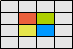
\includegraphics[scale=1]{images/bilinear_interpolation_1}
		\caption{original image \label{bilinear1}}
	\end{figure}

	On \ref{bilinear1} we can see the original image where all pixel are known pixels. Now what happen if we stretch this image 
	from a 2x2 to a 3x3 image?
	
	\begin{figure} [H]
		\centering
		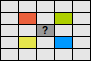
\includegraphics[scale=1]{images/bilinear_interpolation_2}
		\caption{original image \label{bilinear2}}
	\end{figure}

	As we can see, after stretch the image to a desired dimension we create some unknown pixels. To those pixels we can apply the linear interpolation 
	to guess the color intensity we should use based in the color of it's neighbor pixels (not by simply copying the neighbor).

	Example above is not realistic, for several reasons. First of them is that in most of the cases we must fill more than one gap in between known pixels,
	second is that in real cases we consider the pixel in the horizontal and vertical direction, instead of diagonal axis. Third reason is that in the 
	previous example the distance between the unknown pixel to the known pixel were always the same, so a regular division would. 
	Check this other example, a bit more realistic:
	
	\begin{figure} [H]
		\centering
		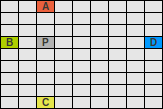
\includegraphics[scale=1]{images/bilinear_interpolation_3}
		\caption{original image \label{bilinear3}}
	\end{figure}
	
	Here we can see that the interpolation cannot be only the mean of the pixel, since the unknown pixel is closer to the point A and B, it's reasonable 
	this unknow pixel receives more red and green color than the other ones.

	Consider \textit{distance(p1,p2)} a function that returns the distance between two pixels, 
	and \textit{color(p1)} a function that returns the color of the pixel p1 . We perform first the Linear interpolation horizontally, so:

	\[ f_h(p)=color(B)*\frac{distance(P,D)}{distance(B,D)}+color(D)*\frac{distance(B,P)}{distance(B,D)}  \]

	We can perform this operation in the vertical axis as well:

	\[ f_v(p)=color(A)*\frac{distance(P,C)}{distance(A,C)}+color(C)*\frac{distance(A,P)}{distance(A,C)}  \]

	Combibing these two approaches we have the bilinear interpolation.

	
\section{Histogram}

	\subsection{Color histogram}

		\textit{Fill me}.

	\subsection{Histogram stretching}

		\textit{Fill me}.

\end{document}
